5. $(x-5)(2y+4x-6)=0\Leftrightarrow\left[\begin{array}{c}x-5=0,\\ 2y+4x-6=0.\end{array}
ight.\Leftrightarrow\left[\begin{array}{c}x=5,\\ y=3-2x.\end{array}
ight.$
$$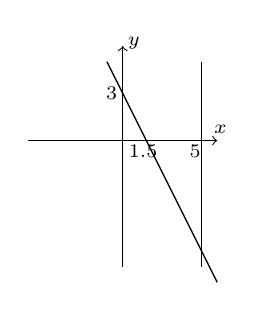
\begin{tikzpicture}[scale=0.2]
\tikzset {line01/.style={line width =0.5pt}}
\tikzset{line02/.style={line width =1pt}}
\tikzset{line03/.style={dashed,line width =0.5pt}}
%\filldraw [black] (0,0) circle (1pt);
\draw [->] (-6,0) -- (6,0);
\draw [->] (0,-8) -- (0,6);
\draw[line01] (5,-8) -- (5,5);
\draw[line01] (-1,5) -- (6,-9);
\draw (6.2,0.7) node {\scriptsize $x$};
\draw (4.6,-0.7) node {\scriptsize $5$};
\draw (1.3,-0.7) node {\scriptsize $1.5$};
\draw (-0.7,3) node {\scriptsize $3$};
\draw (0.7,6.2) node {\scriptsize $y$};
\end{tikzpicture}$$
